% !TeX root = ../main.tex
% Add the above to each chapter to make compiling the PDF easier in some editors.
\chapter{Performance and Evaluation}\label{chapter:performance}
\section{Deployment}\label{deployment}
The version of the Android application deployed during the field testing \parencite{final-version-app} as well as the server version deployed during the field testing \parencite{final-version-server} is hosted on GitHub. The latest version of the same repository provides the same functionality but includes improvements (e.g. bug-fixes, comments, ...) compared to the deployed version. The latest version of all repositories is  also duplicated on our university servers \parencite{lrz}.
The proposed Android application and server have been tested on 16 devices for six days from 30.05.2019 until 04.06.2019. However, evaluating the \textit{lastSeen} timestamp of the users showed that only 13 installations were active after 31.05.2019. The server was deployed in the IBM Cloud as a 128 MB node.js instance, the database was hosted as a free version at mongodb.com.

We ran 7 different aggregation requests defined in Section \ref{data-aggregation-design} covering different time spans from single days to the whole time period. Also, we limited the number of participants in each aggregation to 10. The results can be found in the tables in this Section and are also available in JSON format on GitHub \parencite{github-results}. The results will be discussed in Chapter \ref{results}. The results of the collection of trajectories were modified in order to protect the privacy of all research participants. We used this testing period also to improve the performance of the server as well as the Android application and to find and remove bugs. All improvements are incorporated in the most recent commits of the respective GitHub repositories.

\section{Data Consumption}
As expected, the data consumption of the Android application was low. Some research participants provided information about the app's data usage. Table \ref{data-consumption} shows the 12 collected results of this rather qualitative than quantitative analysis. Screenshots of the provided information are attached in the Appendix. On 75\% of the devices, the data consumption for 6 days was below 21 MB. The highest data consumption was 376 MB and is attributable to an error that occurred on the last day of the testing period. Requests were sent multiple times during the whole period and up to unlimited times on the last day due to this error in combination with another error that was present during the whole time span. This explains the high data consumption reported also by two other participants as the error occurred at least on three devices. The data suggests that the average data consumption in a production environment would be lower and regarding the size of our setup below 100 MB per month. Furthermore, a mobile connection is not required. In the future, the setup can be changed to use only or mostly WIFI connections.
Some few available reports about battery consumption also indicate a rather moderate battery consumption.

\begin{table}[h!]
	\centering
	\begin{tabular}{|l|l|}
		\hline
		\multicolumn{2}{|c|}{\textbf{Combined Data Consumption from 30.05.2019 - 04.06.2019}}                     \\ \hline
		\textbf{Data Consumption} & \multicolumn{1}{c|}{\textbf{Comment}}                       \\ \hline
		0 MB                               & mobile data only, WIFI unknown                              \\ \hline
		2.6 MB                             &                                                             \\ \hline
		6.19 MB                            & mobile data only, WIFI unknown                              \\ \hline
		6.29 MB                            & mobile data only, WIFI unknown                              \\ \hline
		8.18 MB                            &                                                             \\ \hline
		8.5 MB                             & From 01.04.2019 - 04.06.2019 only                           \\ \hline
		11.98 MB                           &                                                             \\ \hline
		18.53 MB                           & 16.5 MB mobile, 2.03 MB WIFI                                \\ \hline
		20.5 MB                            &                                                             \\ \hline
		75.73 MB                           & From 01.04.2019 - 04.06.2019 only, possible error candidate \\ \hline
		49.39 MB                           & mobile data only, WIFI unknown, possible error candidate    \\ \hline
		376 MB                             & Known and fixed error                                       \\ \hline
	\end{tabular}
	\caption{Overall data consumption of the Android application during the testing period.}
	\label{data-consumption}
\end{table}

\section{Aggregation Results}\label{results}
We computed the aggregation over several different time spans. We aggregated the average number of steps across all participants, the average time spent walking, running, in a vehicle or on a bicycle and collected a list of each individual's average number of steps. The results can be seen in Table \ref{results-steps} - \ref{results-biking}. The results from the experimental aggregation of trajectories will be discussed in Chapter \ref{trajectories}.

\subsection{Validity of Results}
Excluding the value for 30.05.2019 where the collection of results started and the data of the fraction of the day prior to the installation is not included, the average time spent walking computed in the aggregations ranges from 52 to 146 minutes per day. Fig. \ref{time-walking-diagram} illustrates the different average values for all computed aggregations. The average time spent walking computed for the whole time span where data from 8 devices is included amounts to 62 minutes and is highlighted in blue. The chart and the exact values depicted in Table \ref{results-walking} suggest that the data itself is consistent: While the average value for aggregations covering the first days is above the overall average, it is mostly below for the second half.

\begin{figure}[h!]
	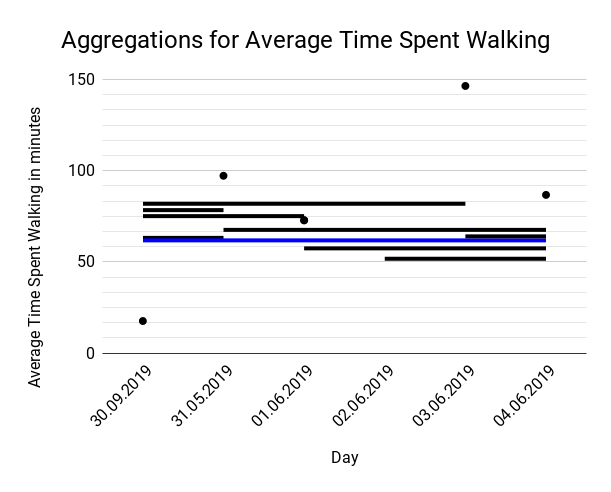
\includegraphics[width=\textwidth]{data/diagrams/average-time-walking2.png}
	\caption{Average time spent walking for covering different time periods.}
	\label{time-walking-diagram}
\end{figure}

At the same time, the reported number of steps per day ranges from 1123 to 4682 per day, excluding outliers (see Table \ref{results-steps}). The average number of steps computed for the whole time span with data from 5 participating devices is 3622. Taking an average speed of roughly 100 steps per minute into account \parencite{steps2}, the results from the average time spent walking and the average number of steps diverge by a factor of 1.7. Considering that apparently, only 6 devices had a step sensor on their phone and the sample size of the steps aggregation is only about half of the sample size of the other aggregations, this deviation does not seem out of range. Furthermore, there was an error computing the number of steps on at least one phone which caused some of the results to be off. Regarding Table \ref{results-steps-listing}, it is clear that the error occurred in the local aggregation process and it seems likely that only on one device this error occurred, as in each aggregation only one value is erroneous.

\begin{table}[]
	\parbox{.45\linewidth}{
		\centering
		\begin{tabular}{|l|l|l|}
			\hline
			\multicolumn{3}{|c|}{\textbf{Average number of steps per day}}          \\ \hline
			\textbf{Time period / Day} & \textbf{N} & \textbf{Value}           \\ \hline
			30.05.2019                 & 5          & 4332                     \\ \hline
			31.05.2019                 & 5          & 3440                     \\ \hline
			01.06.2019                 & 1          & 17                       \\ \hline
			03.06.2019                 & 3          & 455411                   \\ \hline
			04.06.2019                 & 3          & 1123                     \\ \hline
			30.05.2019 - 31.05.2019    & 6          & 3279                     \\ \hline
			30.05.2019 - 31.05.2019    & 5          & 4030                     \\ \hline
			30.05.2019 - 01.06.2019    & 6          & 4271                     \\ \hline
			30.05.2019 - 03.06.2019    & 5          & 643959                   \\ \hline
			30.05.2019 - 04.06.2019    & 5          & 3623                     \\ \hline
			31.05.2019 - 04.06.2019    & 3          & 4681                     \\ \hline
			01.06.2019 - 04.06.2019    & 2          & 2089                     \\ \hline
			02.04.2019 - 04.06.2019    & 3          & 326363                   \\ \hline
			03.04.2019 - 04.06.2019    & 3          & 455904                   \\ \hline
		\end{tabular}
		\caption{Average number of steps per day aggregated across all participating users for different time spans.}
		\label{results-steps}
	}
	\hfill
	\parbox{.45\linewidth}{
		\centering
		\begin{tabular}{|l|l|l|}
			\hline
			\multicolumn{3}{|c|}{\textbf{Average time spent walking {[}min{]}}}          \\ \hline
			\textbf{Time period / Day} & \textbf{N} & \textbf{Value} \\ \hline
			30.09.2019                 & 10         & 17.63                    \\ \hline
			31.05.2019                 & 10         & 97.25                    \\ \hline
			01.06.2019                 & 4          & 72.85                    \\ \hline
			03.06.2019                 & 9          & 146.49                   \\ \hline
			04.06.2019                 & 8          & 86.77                    \\ \hline
			30.05.2019 - 31.05.2019    & 10         & 63.20                    \\ \hline
			30.05.2019 - 31.05.2019    & 10         & 78.41                    \\ \hline
			30.05.2019 - 01.06.2019    & 10         & 75.14                    \\ \hline
			30.05.2019 - 03.06.2019    & 9          & 81.94                    \\ \hline
			30.05.2019 - 04.06.2019    & 8          & 61.86                    \\ \hline
			31.06.2019 - 04.06.2019    & 7          & 67.63                    \\ \hline
			01.06.2019 - 04.06.2019    & 7          & 57.44                    \\ \hline
			02.06.2019 - 04.06.2019    & 7          & 51.75                    \\ \hline
			03.06.2019 - 04.06.2019    & 7          & 64.04                    \\ \hline
		\end{tabular}
		\caption{Average time spent walking (in minutes) aggregated across all participating users for different time spans.}
		\label{results-walking}
	}
\end{table}

The average time spent running depicted in Table \ref{results-running} ranges up to only 2 minutes per day with one day having a 0 value across 8 participating devices. Most likely, only a fraction of the research participants goes running on a regular basis and probably even less take their smartphone along. This assumption reflects the low values for the average time spent running. Especially as attributing the whole average value to one device only would mean that one person conducted a run of fewer than 20 minutes seems unlikely, while it seems likely that quite some persons run for a short amount of time e.g. to catch a train or metro. Nevertheless, we cannot prove this assumption. Furthermore, it highlights that for thorough analysis the aggregation of the mean value is not sufficient.
Similarly, the average number of steps across all participants of an aggregation is not very robust and does not provide much information. Table \ref{results-steps-listing} provides the average number of steps of each individual participating in the request. With the median ranging from 3195 to 3565 in all aggregations with more than 3 valid values and a mean number of 5205 steps in Germany \parencite{steps3} we have no doubt about the correctness of the values except the values resulting from (probably only one) erroneous device.

\begin{table}[]
	\centering
	\begin{tabular}{|l|l|l|}
		\hline
		\multicolumn{3}{|c|}{\textbf{Listing of the average number of steps per day per of each participant}} \\ \hline
		\textbf{Time period / Day}         & \textbf{N}        & \textbf{Values}                          \\ \hline
		30.05.2019                         & 10                & 1661, 1246, 3195, 7714, 7842             \\ \hline
		31.05.2019                         & 10                & 2747, 775, 3924, 9203                    \\ \hline
		01.06.2019                         & 4                 & 17                                       \\ \hline
		03.06.2019                         & 9                 & 914, 1042, 1364278                       \\ \hline
		04.06.2019                         & 8                 & 1103, 13332, 934                         \\ \hline
		30.05.2019 - 31.05.2019            & 10                & 550, 2905, 3195, 775, 8828, 3419        \\ \hline
		30.05.2019 - 31.05.2019            & 10                & 550, 8828, 5145, 3195, 2433              \\ \hline
		30.05.2019 - 01.06.2019            & 10                & 8126, 3195, 283, 8828, 1629, 3565        \\ \hline
		30.05.2019 - 03.06.2019            & 9                 & 598, 3195, 1669, 8828, 3205505           \\ \hline
		30.05.2019 - 04.06.2019            & 8                 & 757, 1719, 8828, 3614, 3195              \\ \hline
		31.05.2019 - 04.06.2019            & 7                 & 757, 9203, 4084                         \\ \hline
		01.06.2019 - 04.06.2019            & 7                 & 826, 33511                               \\ \hline
		02.04.2019 - 04.06.2019            & 7                 & 974691, 1231, 3168                       \\ \hline
		03.04.2019 - 04.06.2019            & 7                 & 1364278, 1231, 2202                      \\ \hline
	\end{tabular}
	\caption{List of the average number of steps per day for each user aggregated for various time spans.}
	\label{results-steps-listing}
\end{table}

\begin{table}[]
	\parbox{.40\linewidth}{
		\centering
		\begin{tabular}{|l|l|l|}
			\hline
			\multicolumn{3}{|c|}{\textbf{Average time spent running {[}min{]}}}          \\ \hline
			\textbf{Time period / Day} & \textbf{N} & \textbf{Value} \\ \hline
			30.09.2019                 & 10         & 1.43                     \\ \hline
			31.05.2019                 & 10         & 1.21                     \\ \hline
			03.06.2019                 & 9          & 1.95                     \\ \hline
			04.06.2019                 & 8          & 0                        \\ \hline
			30.05.2019 - 31.05.2019    & 10         & 1.96                     \\ \hline
			30.05.2019 - 31.05.2019    & 10         & 1.89                     \\ \hline
			30.05.2019 - 01.06.2019    & 10         & 1.73                     \\ \hline
			30.05.2019 - 03.06.2019    & 9          & 1.79                     \\ \hline
			30.05.2019 - 04.06.2019    & 8          & 1.55                     \\ \hline
			31.06.2019 - 04.06.2019    & 7          & 0.83                     \\ \hline
			01.06.2019 - 04.06.2019    & 7          & 0.99                     \\ \hline
			02.06.2019 - 04.06.2019    & 7          & 1.05                     \\ \hline
			03.06.2019 - 04.06.2019    & 7          & 0.16                     \\ \hline
		\end{tabular}
		\caption{Average time spent running (in minutes) aggregated across all participating users for different time spans.}
		\label{results-running}
	}
	\hfill
	\parbox{.50\linewidth}{
		\begin{tabular}{|l|l|l|}
			\hline
			\multicolumn{3}{|c|}{\textbf{Average time spent in a vehicle {[}min{]}}}     \\ \hline
			\textbf{Time period / Day} & \textbf{N} & \textbf{Value} \\ \hline
			30.05.2019                 & 10         & 8.24                     \\ \hline
			31.05.2019                 & 10         & 119.92                   \\ \hline
			01.06.2019                 & 4          & 90.40                    \\ \hline
			03.06.2019                 & 9          & 71.74                    \\ \hline
			04.06.2019                 & 8          & 35.51                    \\ \hline
			30.05.2019 - 31.05.2019    & 10         & 68.40                    \\ \hline
			30.05.2019 - 31.05.2019    & 10         & 90.49                    \\ \hline
			30.05.2019 - 01.06.2019    & 10         & 82.19                    \\ \hline
			30.05.2019 - 03.06.2019    & 9          & 62.16                    \\ \hline
			30.05.2019 - 04.06.2019    & 8          & 59.34                    \\ \hline
			01.06.2019 - 04.06.2019    & 7          & 51.07                    \\ \hline
			31.05.2019 - 04.06.2019    & 7          & 68.20                    \\ \hline
			02.04.2019 - 04.06.2019    & 7          & 48.89                    \\ \hline
			03.04.2019 - 04.06.2019    & 7          & 45.96                    \\ \hline
		\end{tabular}
		\caption{Average time spent in a vehicle (in minutes) aggregated across all participating users for different time spans.}

		\label{results-vehicle}
	}
\end{table}

\begin{table}[]
	\centering
	\begin{tabular}{|l|l|l|}
		\hline
		\multicolumn{3}{|c|}{\textbf{Average time spent biking {[}min{]}}}           \\ \hline
		\textbf{Time period / Day} & \textbf{N} & \textbf{Value} \\ \hline
		30.05.2019                 & 10         & 2.29                     \\ \hline
		01.06.2019                 & 4          & 14.99                    \\ \hline
		03.06.2019                 & 9          & 31.03                    \\ \hline
		04.06.2019                 & 8          & 23.81                    \\ \hline
		30.05.2019 - 31.05.2019    & 10         & 11.10                    \\ \hline
	\end{tabular}
		\caption{Average time spent biking (in minutes) aggregated across all participating users for different time spans.}
	\label{results-biking}
\end{table}

The average time spent in a vehicle (including means of public transport) ranges from 36 to 120 minutes (excluding the aggregation only covering the first day) while the average time spent in a vehicle computed by the aggregation covering the whole time span is 59 minutes. The exact results are depicted in Table \ref{results-vehicle}. The collected trajectories in Section \ref{trajectories} show two rather long trajectories which probably contributed to the high average time of 120 minutes spent in a vehicle in one of the aggregations.

The average time spent biking ranges from 11 to 31 minutes. The aggregation for bicycle use across was erroneous except for some aggregations. Table \ref{results-biking} depicts the few correct aggregations that were obtained. Nevertheless, both aggregations, the time spent biking and the time spent in a vehicle, seem reasonable to us, especially as all participants were active in the Munich area which is  a rather bicycle-friendly city.

\subsection{Explanation of Inconsistency}
The same aggregation covering the time span from 30.05.2019 to 31.05.2019 was computed twice for 4 of the aggregation types. The results show that not only the number of participants varies but also the value varies from 4\% to 18\%. For each aggregation, the selected participants might be different. With a total number of 16 participants in our research, there has to be an intersection. We see the same phenomena of at first glance inconsistent data e.g. regarding the aggregations for the time spent running on 30.05.2019, 31.05.2019 and the aggregation covering both days. The aggregation covering both days yields a higher value than every single aggregation which must originate in a differing underlying research population.
Also, computing the average number of steps from the single collected values in Table \ref{results-steps} yields 3622 and shows that apparently, the same people participated in this aggregation and the aggregation of average values across all participants. At the same time, the aggregation covering 01.6. - 04.06 shows without the need of a calculation that different people participated.
Even though, different underlying research populations produce different results, the deviation in the aggregations is within an acceptable range and will be more robust, when the number of participants is increased. Furthermore, the median value will be even more robust to computing the same aggregation twice.
Fig. \ref{steps-diagram} also supports the findings, that even with a small research population, results are already robust to some extent. The histogram using a bucket size of 1000 in combination with a 20\% outlier percentile shows the average daily steps values obtained from all aggregations compared to the ones obtained only from the aggregation covering the whole time span. Taking the different sample size into account, the distribution of buckets for all aggregations and the distribution of buckets for the aggregation covering the whole time span resemble each other and suggests a certain robustness of the results.

\begin{figure}[h!]
	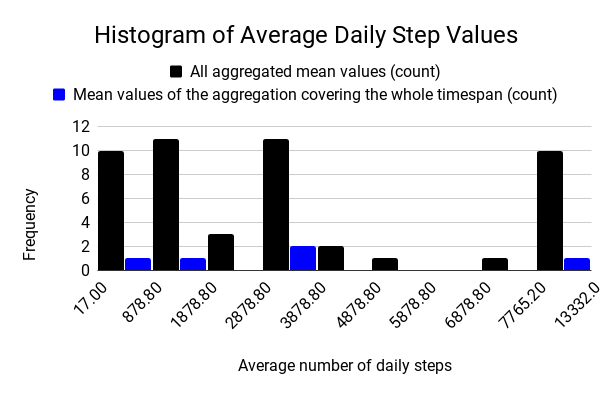
\includegraphics[width=\textwidth]{data/diagrams/daily-step-diagram.png}
	\caption{Histogram showing the average number of daily steps from all aggregations compared to the single aggregation covering the whole time span.}
	\label{steps-diagram}
\end{figure}

\subsection{Inference on Aggregated Data}\label{inference}
Regarding the aggregations computing mean values across all participants, we do not see any possibility to infer information about the users who participated, especially as not even the identifier of the user used by the server is published alongside with the aggregation. In addition, we showed that when repeating the same aggregation request, the user base changes and the value accordingly. Nevertheless, from the two different values for the same aggregation request, we cannot draw any inference. Also, an overlapping time span in the aggregations e.g. 30.05.2019, 31.05.2019 and an aggregation covering both days, as well as the aggregations covering the first two days and the last five days, does not allow for inference in the case of mean values aggregated across all participants.
The collection of individual mean values in Table \ref{results-steps-listing} shows that with a high probability the same participant with an average value of 8828 steps per day who participated in the request covering the first two days also participated in the request covering the whole time span. Based on the information that days with a zero value of the step counter are excluded also locally from the aggregation, we can infer that this person's phone did not register any steps after the first two days, otherwise the value in the second aggregation would have changed. Similarly, we can infer that the user with 757 steps on average per day who participated in the requests covering the whole 6-day time span and the aggregation covering only the last 5 days probably did not register steps on the first day.
In summary, we can only infer information that some users who participated in one aggregation, did or did not participate in another aggregation. As this information is endogenous to our data set, it cannot be used to link this data set to other data sets in order to infer further information.
Assuming that we also had the collected averages of all aggregations and not only of the number of steps, linking different aggregations e.g. the number of steps and the time spent walking would only possible with a limited likelihood due to the following reasons. First, there is no exact match of e.g. time spent walking and number of steps so that always a range of values of another aggregation would fit. Next, we cannot even assure that the same user participated in both different aggregations. Assuming now that there is another data set where e.g. a combination of walked steps and time spent walking is a quasi-identifier as defined by Sweeney \parencite{k-anonymity-achieving}, the likelihood of obtaining a correct link is still low. For example, the number of steps in both data sets would have to be computed with the exact same logic to have a high chance of obtaining a link. And even then, as we mentioned before, we do not see any sensitive information being inferrable from our data set. Apart from that, we can guarantee that the discussed aggregations do not expose raw location data or GPS tracks that are the base of inference attacks on anonymized data sets investigated by former research.

\subsection{Feasibility Analysis of further Aggregations}\label{trajectories}
Using the algorithm described in Chapter \ref{local-data-aggregation}, a total of 406 trajectories were computed from the raw GPS data. The experimental collection of trajectories clearly shows privacy risks as pointed out e.g. by Drakonakis et al. \parencite{cellphone}. Therefore, we only publish a modified result set\footnote{Whenever the trajectory started or ended clearly in a precise private location e.g. housing or work-place, we slightly modified this trajectory so that the results do not represent actual trajectories. Nevertheless, the meaning of the results should not have changed.}. Most of the trajectories are shown in Fig. \ref{trajectories1} and \ref{trajectories2}. The complete results can also be found in the respective repository \parencite{github-results}.

\begin{figure}[h!]
	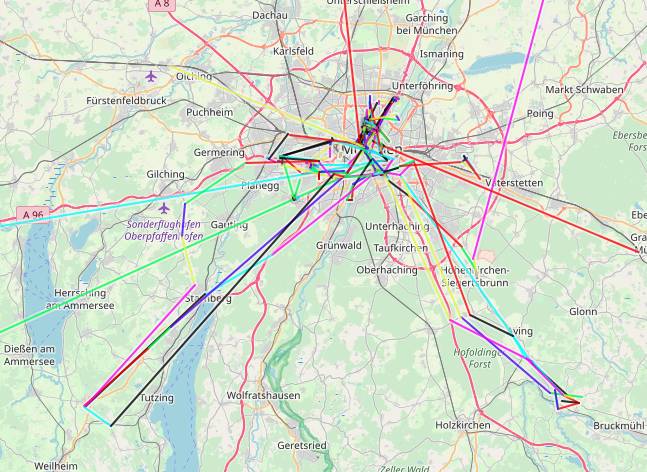
\includegraphics[width=\textwidth]{data/trajectories-2.png}
	\caption{Excerpt of all trajectories in the greater Munich area.}
	\label{trajectories1}
\end{figure}

\begin{figure}[h!]
	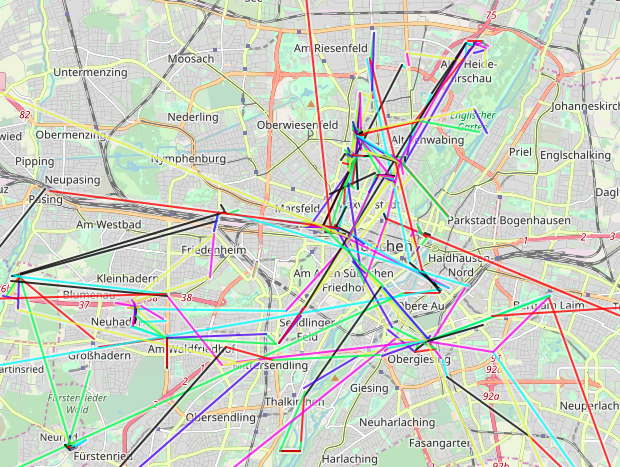
\includegraphics[width=\textwidth]{data/trajectories-3.png}
	\caption{Excerpt of all trajectories inside Munich.}
	\label{trajectories2}
\end{figure}

In more than 90\% of all cases, local trajectories obtained from one of the researchers participating devices could be matched to an activity for more than 90\% of the duration of the trajectory. This data suggests that these trajectories can easily be linked locally and a change of transport system e.g. metro to bicycle can be identified. For example at the locations Giselastraße, Odeonsplatz and central station, many trajectories end or start. Mapping the current activity to those trajectories enables aggregations as mentioned in Chapter \ref{aggregation-schemes}. Noting that locally all GPS points registered during the trajectories are available, it is also easy to compute the distance travelled or infer a more specific activity e.g. on a train, in a bus or in a car. Also, it is possible to compute how many people combine e.g. bicycle and car or public transport within one trajectory and furthermore identify, which station is most likely (in case of public transport) to be combined with using a bicycle.

The trajectories also show that in the not-anonymized data set we had at hands, the enumeration of the trajectories, of which the endpoints often did not clearly indicate an ongoing, indicated that they were indeed connected. This highlights the importance of list order randomization to provide a maximum level of privacy but also shows that our algorithm of finding trajectories still has possibilities for improvement.

In order to see possible improvements like this one, it will always be helpful to have insights into the raw data of some people e.g. the researchers themselves. Nevertheless, some of the insights gained through the trajectories aggregation could also be gained from a similar aggregation that would still not expose the raw data. By aggregating trajectories in a way that only each road that was used is marked as used or not used, a map could be obtained that highlights the areas covered by the data collected through the application.

\section{Further Scenarios}
As mentioned in the introduction, the motivation of this research stems from giving the general public access to data that is currently proprietary to e.g. Google. Google collects location data through its Google Maps application which offers the user high value e.g. through its navigation feature. In order for our approach to offer the user some value, a similar approach could be taken. For example, our approach could be integrated into Open Street Maps.
Nevertheless, a critical and very important feature of e.g. Google Maps is the creation of traffic alerts and respective re-routing. This feature though requires real-time or almost-real-time data. We believe that our approach can still provide privacy to the user while obtaining the necessary data. The average speed on roads (taking different times of the day into account) can be computed through an aggregation based on historical data like the aggregations implemented in our setup. 
Now if a user registers a speed on one road that is significantly lower than normal at this time of the day, the user chooses a random list of users known e.g. through recent aggregations and sends the signal as a request for those users to the server. They randomly according to a fixed percentage choose to inform the server about the traffic jam or forward the signal another time. The signal contains a unique random id thus that the server counts the signal only once even when receiving it multiple times from different users. If more than a threshold of signals are received, a traffic jam is created. Also, the request is not forwarded anymore after a certain time to stop it from spreading unlimited. This way, choosing a probability of sending the signal to the server of e.g. 10\%, 10-anonymity according to Sweeney \parencite{k-anonymity} can be provided. Because traffic jams worth reporting usually last longer than a few minutes, the delay caused through the forwarding should be ok. In addition, not only traffic jams but also road closures could be detected e.g. through the aggregation mentioned at the end of the last Section.